\appendix
\begin{appendices}
\section{Audio pre-processing code}


The following code records, processes and then plays the double integrated and square-rooted output. Additional code sources are available on the github repository for this project at \url{https://github.com/SnoWHandS/Directional_Audio_System}.

\begin{lstlisting}[caption={Record, process and play Julia code}\label{lst:juliarecProPly},language=julia, style=jlcodestyle]

#Developed by Dillon Heald for use with a directional ultrasonic speaker array
#Date: April 2020



using PortAudio, Statistics, PyPlot, FFTW

stream = PortAudioStream(1, 1, blocksize=1024)

offset = 20

A = 1750                       #Amplitude multiple for final output signal
sample_rate = 44100
Nseconds = 10
N = Nseconds * sample_rate
Δt=1/sample_rate                 #seconds: inverse of sample rate
t=(0:N-1)*Δt                    #time axis def
#Define f_axis
Δf=1/(N*Δt)
f=0:(N-1)*Δf
#create array of freq values stored in f_axis. First element maps to 0Hz
if mod(N,2)==0    # case N even
    f_axis = (-N/2:N/2-1)*Δf;    
else   # case N odd
    f_axis = (-(N-1)/2 : (N-1)/2)*Δf; 
end

#Function for integrating a signal via Riemann sums
function integrate(x, Δt)
    N=length(x)
    y=zeros(N);
    for n=2:N
        y[n]=x[n-1]*Δt + y[n-1]
    end
    return y
end

#Function for high pass filtering a time domain
function hpf(in_signal, time_step, cutoff_freq)
    out_signal = Array{Float64}(undef, length(in_signal));
    RC = 1/(2*pi*cutoff_freq);
    a = RC/(RC + time_step);
    out_signal[1] = in_signal[1]
    for i = 2:length(in_signal)
        out_signal[i] = a*(out_signal[i-1] + in_signal[i] - in_signal[i-1]);
    end;
    return out_signal;
end;

println("Recording $(Nseconds) seconds of sampled audio")

buf_read = read(stream,N)
buf = buf_read

println("Processing $(Nseconds) seconds of sampled audio")

#Shift function to above 0 for preprocessing
buf = buf_read

#integrate once with function centered at 0
y1 = integrate(buf, Δt)
Y1 = fft(y1)
y1_filt = hpf(y1,Δt,80)
Y1_filt = fft(y1_filt)
#integrate twice
y2 = integrate(y1_filt, Δt)
Y2 = fft(y2)
y2 = hpf(y2,Δt,160)
y2_filt = hpf(y2,Δt,160)
Y2_filt = fft(y2_filt)

#Shift function to above 0 for preprocessing
buf = y2_filt.-minimum(y2_filt)

#Perform a square root of the samples
buf = sqrt.(buf)

close("all")
figure(2)
nStart=Int(round(Δt/Δt))
nEnd=Int(round(N*Δt/Δt))
subplot(3,1,1)
plot(t[nStart:nEnd],y1_filt[nStart:nEnd])
xlabel("y1 output")
subplot(3,1,2)
plot(f_axis,abs.(fftshift(Y1)))
xlabel("FFT of Y1")
subplot(3,1,3)
plot(f_axis,abs.(fftshift(Y1_filt)))
xlabel("FFT of Y1 filtered")

figure(3)
nStart=Int(round(Δt/Δt))
nEnd=Int(round(N*Δt/Δt))
subplot(3,1,1)
plot(t[nStart:nEnd],y2_filt[nStart:nEnd])
xlabel("y2 output")
subplot(3,1,2)
plot(f_axis,abs.(fftshift(Y2)))
xlabel("FFT of Y2")
subplot(3,1,3)
plot(f_axis,abs.(fftshift(Y2_filt)))
xlabel("FFT of Y2 filtered")

#filter away DC
buf = hpf(buf,Δt,75)

#shift center back to 0 and amplify to be audible
buf = A*buf

BUF = fft(buf)
BUF_READ = fft(buf_read)

figure(1)
nStart=Int(round(0.0025/Δt))        #Artifact with samples before 0.0025s = 2.5ms
nEnd=Int(round(N*Δt/Δt))
subplot(4,1,1)
plot(t[nStart:nEnd],buf[nStart:nEnd])
xlabel("envelope output")
subplot(4,1,2)
plot(t[nStart:nEnd],buf_read[nStart:nEnd])
xlabel("original output")
subplot(4,1,3)
plot(f_axis,abs.(fftshift(BUF_READ)))
xlabel("FFT of original")
subplot(4,1,4)
plot(f_axis,abs.(fftshift(BUF)))
xlabel("FFT of output")


println("Playing $(Nseconds) seconds of sampled audio")

write(stream, buf)
close(stream)

\end{lstlisting}

\section{Project management \& planning}
The following project planning was performed following initial proposal of the project. By mid March, the Covid-19 pandemic struck South Africa and resulted in national lock down. This altered the scope of the project and shifted timelines, thus the date information is not accurate; however, the work flows remained the same albeit shifted and reduced in scope to account for the disruption.
\subsection{Work breakdown structure}
\begin{figure}[ht]
    \centering
    \includegraphics[width=\textwidth]{Figures/Work_Breakdown_Structure_1000dpi.png}
    \caption{Work breakdown structure for the the directional audio system}
    \label{fig:wbs}
\end{figure}
\newpage
\subsection{Gantt chart}
\begin{figure}[ht]
    \centering
    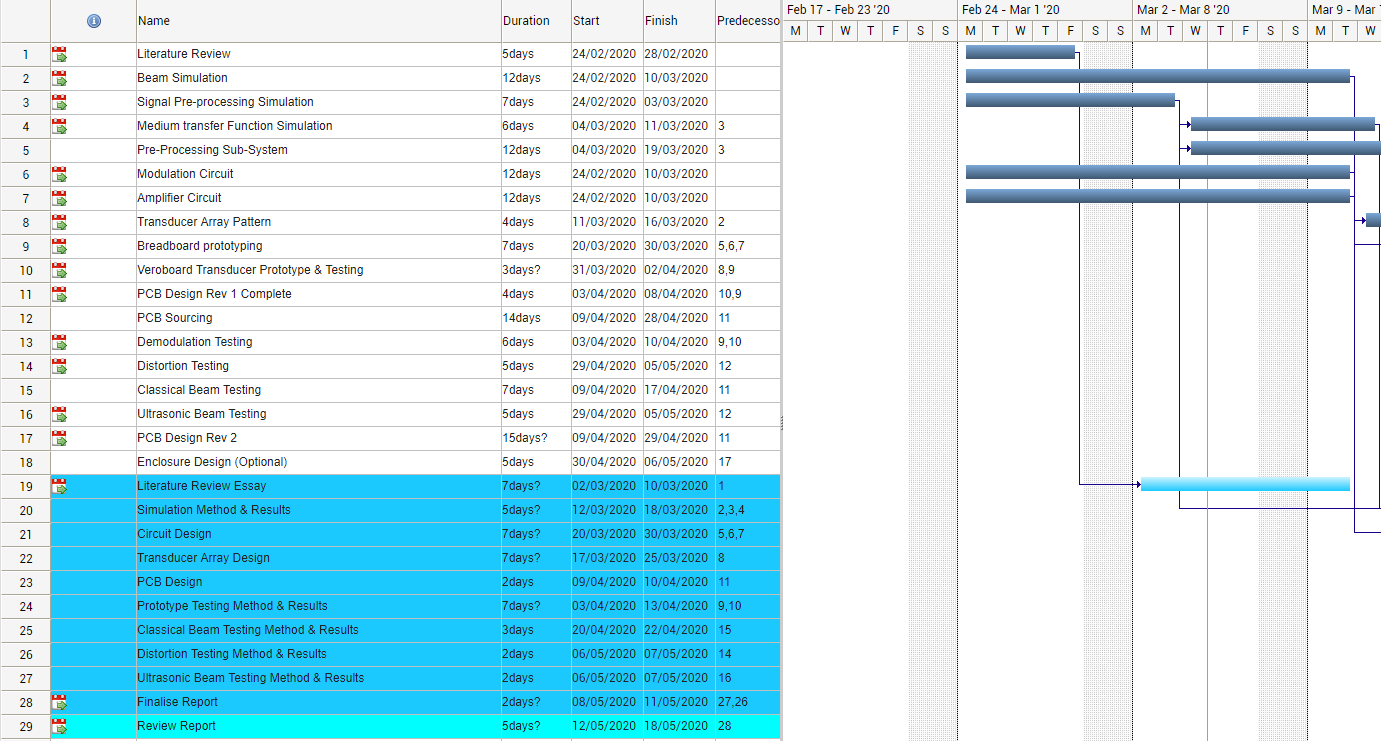
\includegraphics[width=\textwidth]{Figures/Gantt1.PNG}
    \caption{Gantt chart part 1}
    \label{fig:gantt1}
\end{figure}
\begin{figure}[ht]
    \centering
    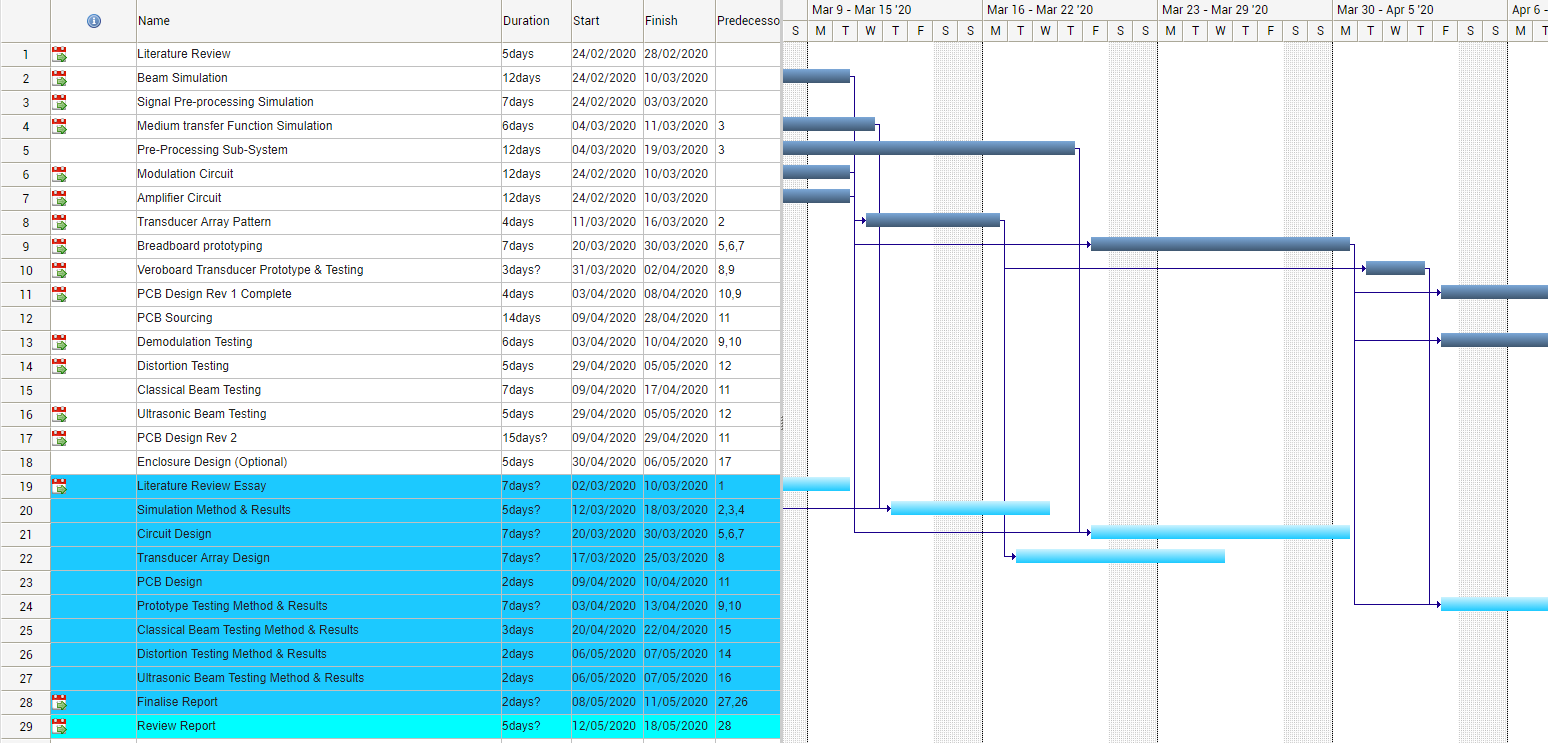
\includegraphics[width=\textwidth]{Figures/Gantt2.PNG}
    \caption{Gantt chart part 2}
    \label{fig:gantt2}
\end{figure}
\begin{figure}[ht]
    \centering
    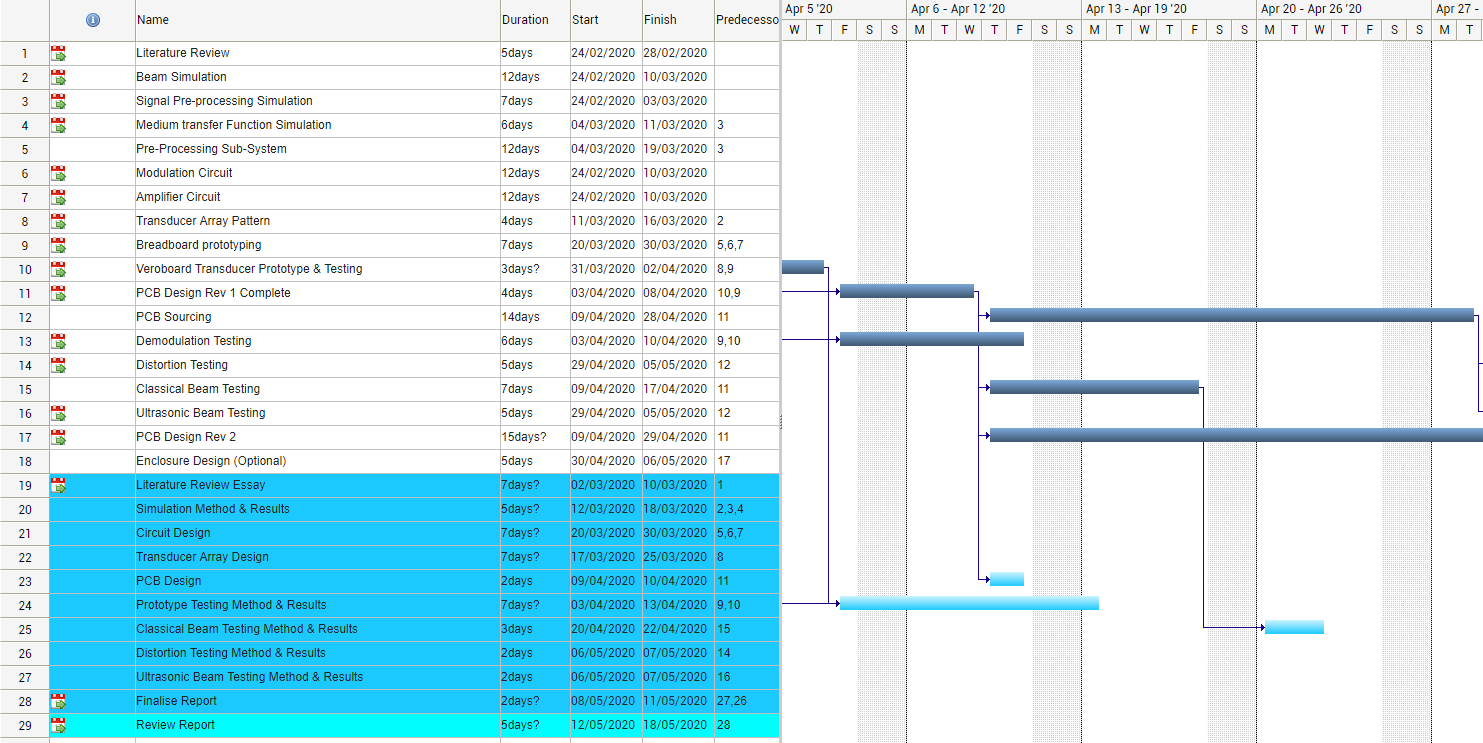
\includegraphics[width=\textwidth]{Figures/Gantt3.PNG}
    \caption{Gantt chart part 3}
    \label{fig:gantt3}
\end{figure}
\begin{figure}[ht]
    \centering
    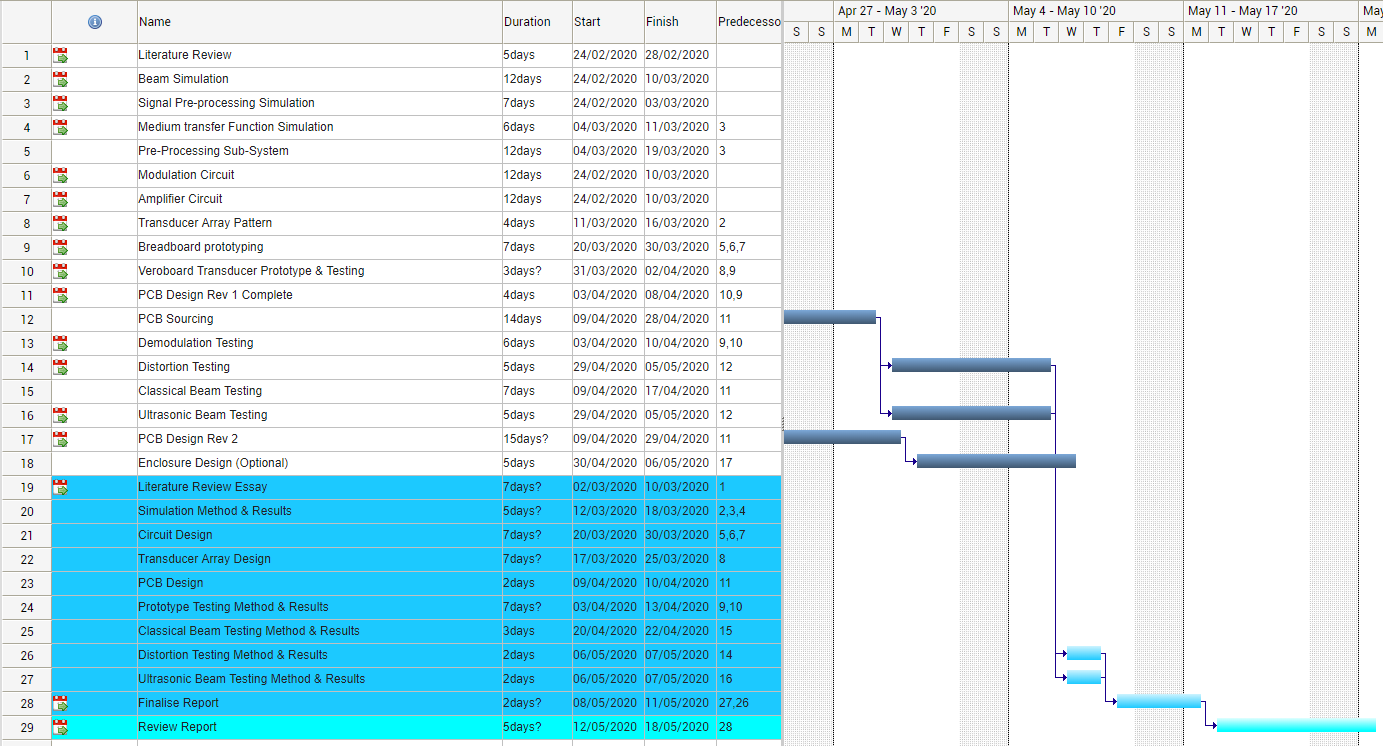
\includegraphics[width=\textwidth]{Figures/Gantt4.PNG}
    \caption{Gantt chart part 4}
    \label{fig:gantt4}
\end{figure}

\clearpage

\section{Beam pattern simulation code}
Note, the code used for beam pattern simulation does not translate the $\omega$ axis to a $\theta$ axis. However, this can be done by performing some of the following changes.\\
Let $\Delta x$ be the sample spacing and N be the number of samples. Considering that our sampled DFT array has indices k=0,1,2.. where each is the the frequency index. In the FFT array, the sample spacing is $\Delta f=\frac{1}{N\Delta x}$.\\
Since $f=k\Delta f$ with $\Delta f = \frac{1}{N\Delta x}$ the $\theta$ axis can be defined by $\theta = sin^{-1}(k\Delta f \lambda)$.
Note however, this is only valid for $\left|f \lambda \right | < 1 $ or $\left |f\right | < \frac{1}{\lambda} $ with angular range $-\frac{\pi}{2}<\theta<\frac{\pi}{2}$ which results in a frequency range of $-\frac{1}{\lambda} < f < \frac{1}{\lambda}$ since the arcsine function outside these bounds will give an error.\\

%f=k*df where k=0,1,2,..

%df = 1/(N*dx)

%Theta = asin( f*lambda)


%which is the angular range from -π/2<θ<π/2   (-90,+90)
%or equivalently ove frequency range -1/λ<f<1/λ
%Outside this range, the asin function will give an error.
%
%In Julia, arrays are indexed starting at 1, so f=(i-1)Δx where i is the
%julia index.
The following code shown in listing \ref{lst:hexpackedSimCode} demonstrates the Julia code used to create the beam shape plots without the above mentioned axis change. This version is for the hexagonally packed array, however; another version of the code for the square packed array is available in the project repository at \url{https://github.com/SnoWHandS/Directional_Audio_System}.
\begin{lstlisting}[caption={Beam pattern simulation code for hexagonally packed array}\label{lst:hexpackedSimCode},language=julia, style=jlcodestyle]
# Script to calculate beam pattern from aperture distribution
# 2D FFT Method
# AJW & DH 2020-05-08
#
# To do: relate frequency domain to angle and label plot axes.
using FFTW

# Define a matrix of points to hold the aperture.
dx = 1.0
dy = dx
# Making N bigger implements zero-padding for finer other-domain spacing.
N=1024;   
# A holds the aperture distribution (e.g. Sound pressure level or E field strength)
A=zeros(N,N);   
x_axis = 0:dx:(N-1)*dx
y_axis = 0:dy:(N-1)*dy

function fill_circle(x0,y0,r0,fill_value,A)
# This function fills a circle, centres (x0,y0) of radius r
# with ones inside matrix A
# Array A is passed by reference
(Ncols,Nrows)=size(A)

i0=x0/dx
j0=y0/dy
iStart=Int(round(i0-(r0/dx+1)))
iEnd=Int(round(i0+(r0/dx+1)))
jStart=Int(round(j0-(r0/dy+1)))
jEnd=Int(round(j0+(r0/dy+1)))

for i=iStart:iEnd; 
  for j=jStart:jEnd
    x = i*dx
    y = j*dy
    R = sqrt( (x-x0)^2 + (y-y0)^2 )
    if R<=r0
      A[i,j]=fill_value
    end
  end
end

end

function createArray(x1,y1,r1)
  (Ncols,Nrows)=size(A)
  for i=1:Ncols; 
       for j=1:Nrows
         x = i*dx
         y = j*dy
         R = sqrt( (x-x1)^2 + (y-y1)^2 )
         if R<=r0
           fill_circle(x0,y0,r0,fill_value,A)
         end
       end
  end
end
#define dimensions of the square grid
dimx=7  #2x2 = 18 3x3 = 9  9x9 = 18/8
dimy=7
offset=1.25 #accounts for the external radius of the transducer
# Fill Aperture matrix with one circular object
ApetureDia = 13.7
r0= ApetureDia/2   #interior radius = 13.7/2 = 6.85mm
x0=N/4;  
y0=N/4;
fill_value=1;
transducerDia = 16.2

elementSpacing = transducerDia - 0.7
wavelength=(343/40000)*1000;  #in mm
# d sin(theta) = lambda -> around 30.3
First_grating_lobe_angle_deg = asin(wavelength/elementSpacing)/pi*180  
println("First_grating_lobe_angle_deg = $(First_grating_lobe_angle_deg), deg")

xmid = x0 + (dimx-1)*sqrt(3)*elementSpacing/2
ymid = y0 + (dimy-1)*elementSpacing/2
#array_radius = (xmid-x0) + elementSpacing/2
array_radius = 41
for i=0:dimx-1
  for j=0:dimy-1
      x1 = x0+(i*sqrt(3)*elementSpacing)
      y1 = y0+(j*elementSpacing)
      radial_distance = sqrt((x1-xmid)^2+(y1-ymid)^2)
      if radial_distance <= array_radius 
         fill_circle(x1,y1,r0,fill_value,A)
      else
          #fill_circle(x1,y1,r0,0.25,A)
      end
      x1 = x1 + sqrt(3)*elementSpacing/2
      y1 = y1 + elementSpacing/2
      radial_distance = sqrt((x1-xmid)^2+(y1-ymid)^2)
      if radial_distance <= array_radius 
         fill_circle(x1,y1,r0,fill_value,A)
      else
        #fill_circle(x1,y1,r0,0.5,A)
      end
  end
end
#fill_circle(xmid,ymid,r0/2,2,A)

B = fftshift(abs.(fft(A)))   # beam pattern
#close("all")
# PyPlot commands (One can also use Plots with plotly backend)
if(false)
using PyPlot
figure(1)
mycolormap = "jet"  # "hsv" "grey" etc. "jet", "
imshow(A); colorbar()
figure(2)
imshow(B, cmap=mycolormap); colorbar()
figure(3)
surf(A, cmap=mycolormap)
figure(4)
surf(B, cmap=mycolormap)
figure(5)
surf(20*log10.(B .+ maximum(B)/10000), cmap=mycolormap)
end

# Plots commands for plotly() backend - uses OpenGL graphics
if(true)
using Plots  # takes 60s to first plot, but worth the wait!

plotly()    # Plot appears in browser window
#gr()
#pyplot()

heatmap(A, size = (1440, 900),reuse=false)
gui()


heatmap(B,size = (1440, 900), reuse=false)
gui()
surface(A, size = (1440, 900),reuse=false)
gui()

surface(B, size = (1440, 900), reuse=false)
gui()
#=
surface(20*log10.(B .+ maximum(B)/10000), color=cgrad([:red,:blue]), reuse=false)
gui()=#
end
\end{lstlisting}


\end{appendices}
